\documentclass[a4paper,11pt]{article}
\input{/home/tof/Documents/Cozy/latex-include/preambule_lua.tex}
\newcommand{\showprof}{show them}  % comment this line if you don't want to see todo environment
\fancyhead[L]{Formation Python}
\newdate{madate}{08}{12}{2020}
\fancyhead[R]{\displaydate{madate}} %\today
%\fancyhead[R]{Seconde - SNT}
%\fancyhead[R]{Première - NSI}
%\fancyhead[R]{Terminale - NSI}
\fancyfoot[L]{~\\Christophe Viroulaud}
\AtEndDocument{\label{lastpage}}
\fancyfoot[C]{\textbf{Page \thepage/\pageref{lastpage}}}
\fancyfoot[R]{\includegraphics[width=2cm,align=t]{/home/tof/Documents/Cozy/latex-include/cc.png}}

\begin{document}
\begin{Form}
\section{Python}
\subsection{Contexte}
Python n'est pas juste un langage d'enseignement. Il est très utilisé dans plusieurs domaines. Un exemple parmi d'autres, le groupe EDF recrute des mathématiciens pour construire divers algorithmes qui sont ensuite codés en Python car simple et rapide d'apprentissage.
\subsection{Syntaxe}
En Python, c'est \emph{l'indentation} qui délimite les blocs de code. Il est d'usage d'indenter par quatre espaces.
\begin{code}[!h]
\begin{lstlisting}
temperature = 8
if temperature < 5:
	print("Mets une écharpe!")
	print("Et un bonnet!")
\end{lstlisting}
\captionof{code}{Deux lignes dans le bloc}
\label{indent1}
\end{code}
\begin{code}[!h]
\begin{lstlisting}
temperature = 8
if temperature < 5:
	print("Mets une écharpe!")
print("Et un bonnet!")
\end{lstlisting}
\captionof{code}{Une ligne dans le bloc}
\label{indent2}
\end{code}


\begin{activite}
Écrire les codes \ref{indent1} et \ref{indent2} et observer les différences d'exécution.
\end{activite}
\begin{framed}
\textbf{Erreur courante:} Les EDI (\emph{Environnement de Développement Intégré)} autorise l'utilisation de la tabulation pour créer l'indentation. Cependant en copiant-collant du code externe (depuis le web par exemple), il est possible de mélanger accidentellement espaces et tabulations et de provoquer une erreur pas toujours évidente à déceler.
\end{framed}
\subsection{Usages}
Les usages décrits ci-après n'ont aucun caractère obligatoire. Ils assurent cependant une cohérence dans les pratiques.\\

Même s'il est possible de le faire en Python (encodage UTF-8), il est conseillé de ne pas utiliser de caractère accentué dans les noms de variables.
\begin{code}[!h]
\begin{lstlisting}
température = 8 # possible mais non conseillé
temperature = 8 # préférable
\end{lstlisting}
\captionof{code}{Éviter les caractères accentués}
\label{accent}
\end{code}

Pour écrire le nom d'une variable, il est d'usage en Python d'utiliser le \emph{snake\_case} plutôt que le \emph{CamelCase} (code \ref{casse}).
\begin{code}[!h]
\begin{lstlisting}
ma_temperature = 8 # snake_case: pas de majuscule et tiret bas
MaTemperature = 8 # CamelCase: majuscule pour chaque mot
\end{lstlisting}
\captionof{code}{Les casses}
\label{casse}
\end{code}
\section{Constructions élémentaires}
\subsection{Variable}
Python est un \emph{langage interprété} c'est à dire que les instructions sont traduites en langage machine \emph{à la volée}. C'est \emph{l'interpréteur} (figure \ref{console}) qui joue ce rôle.
\begin{figure}[!h]
\centering
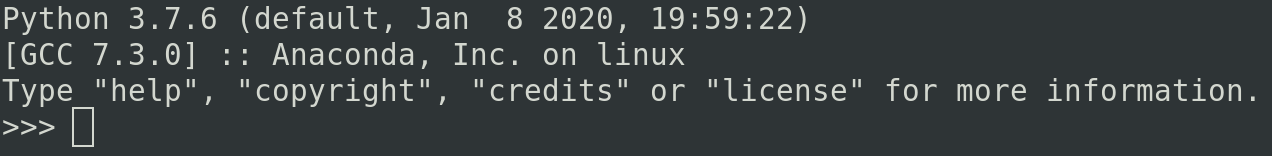
\includegraphics[width=10cm]{ressources/console.png}
\captionof{figure}{Console Python}
\label{console}
\end{figure}
\begin{activite}
\begin{enumerate}
\item Dans le dossier \emph{Maths} ou \emph{NSI} du bureau, ouvrir une console Python: \emph{Python 3.6.8}
\item Entrer les instructions ci -après (valider après chaque ligne):
\begin{lstlisting}
a = 12
b = 17
c = a + b
c
\end{lstlisting}
\end{enumerate}
\end{activite}
\begin{aretenir}[Erreur courante]
Le signe \textbf{=} n'est pas à comprendre au sens mathématique. C'est un signe d'affectation. Ainsi l'instruction
\begin{lstlisting}
12 = a
\end{lstlisting}
est juste mathématiquement mais ne signifie rien en Python.
\end{aretenir}
En première approche, nous pouvons considérer une \emph{variable} comme une boîte qui contient une information Cette information peut être de plusieurs natures (nombre, texte, tableau...)
\subsection{Types de données}
\subsubsection{Typage}
Les données utilisées dans un programme peuvent être de différentes natures. Une \emph{chaîne de caractère} permettra l'affichage d'un message à l'écran alors qu'un \emph{entier} sera permettra d'effectuer un calcul.
\subsubsection{Typage dynamique}
Dans un programme, une variable possède un type déterminé par son contenu. La fonction Python \emph{type()} donne le type d'une variable.
\begin{lstlisting}
a = 42
type(a)
\end{lstlisting}
Ce code retourne \emph{int} pour \emph{integer (entier)}.\\
En Python il est possible de changer le type d'une variable.
\begin{activite}
Tester le code:
\begin{lstlisting}
a = 42
type(a)
a = "test"
type(a)
\end{lstlisting}
\end{activite}
\subsubsection{Les types de base}
\begin{itemize}
\item \textbf{int:} \emph{integer}; nombre entier (42)
\item \textbf{str:} \emph{string}; chaîne de caractère ("test")
\item \textbf{bool:} \emph{boolean}; valeur booléenne (True ou False)
\item \textbf{float:} \emph{flottant}; nombre à virgule flottante (4.2)
\end{itemize}
\begin{aretenir}[Erreurs courantes]
\begin{itemize}
\item La souplesse de Python qui permet de changer le type d'une variable, est perçue par certains comme une source d'erreur potentielle. D'une manière générale on évitera cette pratique.
\item La représentation en mémoire des nombres flottants est source de confusion. Dans la console, tester le code:
\begin{lstlisting}
0.1 + 0.2
\end{lstlisting}
Le résultat peut paraître déroutant. Ainsi la comparaison
\begin{lstlisting}
0.1 + 0.2 == 0.3
\end{lstlisting}
renvoie \emph{False}. \textbf{D'une manière générale, il ne faut pas comparer deux nombres flottants.}
\end{itemize}
\end{aretenir}
\begin{activite}
Tester les instructions ci-après et expliquer ce qu'elles renvoient.
\begin{lstlisting}
20/3
20//3
20%3
\end{lstlisting}
\end{activite}
\subsection{Input/Output}
\subsubsection{Entrée}
L'instruction
\begin{lstlisting}
input()
\end{lstlisting}
demande une valeur à l'utilisateur. Cependant la valeur est inaccessible. Il faut donc la stocker dans une variable en mémoire:
\begin{lstlisting}
age = input()
\end{lstlisting}
Pour être plus explicite, il est possible d'ajouter un \emph{prompt}.
\begin{lstlisting}
age = input("Entrez votre âge: ")
\end{lstlisting}
\begin{aretenir}[Erreur courante]
La fonction \emph{input()} renvoie systématiquement une chaîne de caractère même si un nombre est entré. Pour convertir la chaîne de caractère en entier (int) ou réel (float), il faut utiliser respectivement les fonction \emph{int()} et \emph{float()}.
\begin{lstlisting}
age = int(input("Entrez votre âge: "))
\end{lstlisting}
\end{aretenir}
\subsubsection{Sortie}
L'instruction
\begin{lstlisting}
print("mon texte")
\end{lstlisting}
affiche \emph{mon texte} à l'écran. 

Il est possible d'afficher le contenu d'une variable:
\begin{lstlisting}
print(age)
\end{lstlisting}
Il ne faut alors pas mettre de guillemets.
Pour combiner texte et variable il existe plusieurs syntaxes.
\begin{code}[!h]
\begin{lstlisting}
# Concaténation
print("Vous avez"+"15 ans")
# La fonction format remplace les accolades par les variables.
print("Vous avez {} ans".format(age))

# Une autre possibilité (pour Python > 3.6). Il faut remarquer le f en début.
print(f"Vous avez {age} ans")
\end{lstlisting}
\captionof{code}{Associer chaîne de caractère et variable}
\label{moncode}
\end{code}
\begin{aretenir}[Erreur courante]
Le code \ref{concatenation} renvoie une erreur.
\begin{center}
\begin{lstlisting}
age = 25
print("Vous avez "+ age +" ans")
\end{lstlisting}
\captionof{code}{Erreur de concaténation}
\label{concatenation}
\end{center}
Il n'est pas possible de concaténer un \emph{String} avec un autre type de données. Il faut d'abord convertir la variable avec la fonction \emph{str()}.
\begin{center}
 \begin{lstlisting}
age = 25
print("Vous avez "+ str(age) +" ans")
 \end{lstlisting}
 \captionof{code}{Conversion en String}
 \label{moncode}
 \end{center} 
\end{aretenir}
\begin{activite}
Écrire un programme qui demande l'âge de l'utilisateur, calcule l'année de naissance et affiche cette année.
\end{activite}
\subsection{Utilisation d'un EDI}
Il peut rapidement être fastidieux d'écrire un programme dans la console Python. Un \emph{Environnement de Développement Intégré} permettra d'écrire plusieurs lignes de code puis se chargera d'envoyer toutes ces lignes à l'interpréteur. De plus, il sera possible d'enregistrer le programme dans un fichier.
\begin{activite}
\begin{enumerate}
\item Créer un dossier \emph{formation-python} dans l'espace personnel de l'ordinateur.
\item Ouvrir un EDI au choix: Spyder, Pyzo, EduPython. Les descriptions ci-après se feront sur Spyder.
\item Écrire le programme de l'activité 4 dans la partie gauche de l'EDI.
\item Enregistrer le programme dans le dossier \emph{formation-python} sous le nom \emph{naissance.py}
\item Exécuter le programme en cliquant sur la flèche verte (figure \ref{execution}) ou en appuyant sur la touche \emph{F5}. Le code est exécuté dans la console en bas à droite.
\end{enumerate}
\end{activite}
\begin{figure}[!h]
\centering

\includegraphics[width=1cm]{ressources/execution.png}
\captionof{figure}{Exécuter un programme}
\label{execution}
\end{figure}
\subsection{Structure conditionnelle}
L'instruction
\begin{lstlisting}
a == b
\end{lstlisting}
renvoie \emph{True} si les variables \emph{a} et \emph{b} sont égales, \emph{False} sinon. 
\\
L'instruction
\begin{lstlisting}
if a == b:
    print(a)
\end{lstlisting}
compare \emph{a} et \emph{b} et affiche \emph{a} \textbf{si a == b}.
\begin{aretenir}[Erreur courante]
Il faut noter l'emploi du \emph{double égal} pour ne pas confondre avec le signe d'affectation.
\end{aretenir}
\begin{activite}
\begin{enumerate}
\item Tester les codes ci-après:
\begin{lstlisting}
a = 5
b = 3
if a == b:
    print("a vaut ",a)
    print("b vaut ",b)
\end{lstlisting}
\begin{lstlisting}
a = 5
b = 3
if a == b:
    print("a vaut ",a)
print("b vaut ",b)
\end{lstlisting}
\item Noter les différences d'exécution.
\item Tester le code ci-après pour plusieurs valeurs de \emph{a} et \emph{b}. Bien observer l'indentation.
\begin{lstlisting}
a = 5
b = 3
if a == b:
    print("a et b sont égaux.")
else:
    print("a et b sont différents.")
\end{lstlisting}
\item Il est possible de tester plusieurs conditions. Trouver des valeurs de \emph{a} et \emph{b} pour lesquelles le message \guill{a est vraiment très grand.} est affiché.
\begin{lstlisting}
a = 5
b = 3
if a == b:
    print("a et b sont égaux.")
elif a > 10*b:
    print("a est vraiment très grand.")
else:
    print("a et b sont différents.")
\end{lstlisting}
\item Enregistrer le programme sous le nom \emph{condition.py}
\end{enumerate}
\end{activite}
\subsection{Répéter une instruction}
\subsubsection{Boucle non bornée}
Une boucle \emph{non bornée} répète une instruction \emph{tant que (while)} la condition est vérifiée.
\begin{activite}
\begin{enumerate}
\item Tester le programme ci-après:
\begin{lstlisting}
compteur = 10
while compteur > 0:
    print("Boum dans {} secondes.".format(compteur))
    compteur = compteur - 1
print("Boum")
\end{lstlisting}
\item À quelle ligne compare-t-on le compteur avec la valeur limite?
\item Quel est le rôle de la ligne 4? Que se passera-t-il si cette ligne est retirée?
\item Enregistrer le programme sous le nom \emph{boucle-non-bornee.py}
\end{enumerate}
\end{activite}
\begin{aretenir}[Erreur courante]
Dans une boucle \emph{while} il faut gérer manuellement le cas où la condition ne sera plus vérifiée. Il arrive régulièrement d'oublier de modifier la valeur du \emph{compteur}. La boucle tourne alors indéfiniment.
\end{aretenir}
\subsubsection{Boucle bornée}
Il existe une autre manière de répéter des instructions avec un mécanisme qui varie le compteur automatiquement.
\begin{activite}
\begin{enumerate}
\item Tester le programme ci-après:
\begin{lstlisting}
for compteur in range(10):
   print("Le compteur vaut {}".format(compteur))
\end{lstlisting}
\item Lire la documentation de la fonction \emph{range}:
\begin{center}
\url{https://docs.python.org/fr/3/tutorial/controlflow.html#the-range-function}
\end{center}
\item Adapter le code précédent pour afficher:
\begin{itemize}
\item Le compteur vaut 6.
\item Le compteur vaut 7.
\item Le compteur vaut 8.
\item Le compteur vaut 9.
\end{itemize}
\item Adapter le code précédent pour afficher:
\begin{itemize}
\item Le compteur vaut 0.
\item Le compteur vaut 3.
\item Le compteur vaut 6.
\item Le compteur vaut 9.
\end{itemize}
\item Enregistrer le programme sous le nom \emph{boucle-bornee.py}
\end{enumerate}
\end{activite}
\begin{aretenir}[Erreur courante]
L'appel \emph{range(10)} renvoie 10 valeurs \textbf{en commençant par 0}. La borne supérieure (10) n'est donc pas dans l'intervalle.
\end{aretenir}
\subsection{Types construits de données}
Pour stocker plusieurs valeurs, il existe plusieurs types de structures.
\subsubsection{Tuple}
Un \emph{tuple} est une séquence \textbf{ordonnée} de plusieurs éléments. En mathématiques on parle de \emph{p-uplet}.
\begin{code}[!h]
\begin{lstlisting}
mon_tuple = (8, 5, 3, 9, 1, 0, 2)
\end{lstlisting}
\captionof{code}{Créer un tuple en Python}
\label{tuple1}
\end{code}

On ne peut modifier un tuple: on dit qu'il est \emph{immuable} ou \emph{non mutable}. Par contre il est possible d'accéder aux éléments individuellement.
\begin{code}[!h]
\begin{lstlisting}
print(mon_tuple[0]) # renvoie 8
\end{lstlisting}
\captionof{code}{Accéder à l'élément de rang 0}
\label{acces}
\end{code}

Le code \ref{acces} renvoie la première valeur du tuple. \textbf{L'indexation commence à 0.}
\subsubsection{Tableaux}
Un deuxième type de structure semble plus adapté lorsqu'on veut stocker des valeurs de manière séquentielle: \emph{les tableaux}. En Python on parle de \emph{list} pour évoquer ces structures.
\begin{code}[!h]
\begin{lstlisting}
mon_tableau = [8, 5, 3, 9, 1, 0, 2]
\end{lstlisting}
\captionof{code}{Créer un tableau}
\label{tableau}
\end{code}

Pour accéder a un élément, la syntaxe est la même que pour les tuples.
\begin{code}[!h]
\begin{lstlisting}
print(mon_tableau[0]) # renvoie 8
\end{lstlisting}
\captionof{code}{Accéder au premier élément}
\label{accestab}
\end{code}

Les tableaux sont \emph{mutables}. Il est possible de modifier leur contenu, ajouter voire supprimer un élément.\begin{center}
\begin{lstlisting}
mon_tableau[2] = 19
\end{lstlisting}
\captionof{code}{Modification du troisième élément}
\label{modif}
\end{center}

\begin{code}[!h]
\begin{lstlisting}
mon_tableau.append(12)
\end{lstlisting}
\captionof{code}{Ajouter un élément en fin de liste}
\label{ajout}
\end{code}

Il existe de nombreuses autres méthodes pour manipuler les tableaux. La documentation Python présente ces outils.
\begin{center}
\url{https://docs.python.org/fr/3/tutorial/datastructures.html}
\end{center}
\subsubsection{Dictionnaires}
Un dictionnaire associe une \emph{clé} à une \emph{valeur}. Il n'y a pas de notion d'indice comme pour les autres types construits.
\begin{code}[!h]
\begin{lstlisting}
dico_identite = {"nom": "Viroulaud", "prenom": "Christophe", "age": 43}
\end{lstlisting}
\captionof{code}{Construction d'un dictionnaire}
\label{moncode}
\end{code}
\begin{code}[!h]
\begin{lstlisting}
print(dico_identite["prenom"]) # renvoie Christophe
\end{lstlisting}
\captionof{code}{Accéder à la valeur associée à la clé \emph{prenom}}
\label{moncode}
\end{code}
\begin{code}[!h]
\begin{lstlisting}
dico_identite["age"] = 25
\end{lstlisting}
\captionof{code}{Modifier une valeur}
\label{moncode}
\end{code}
\subsubsection{Parcourir un type construit de données}
Les types construits sont \emph{itérables}. Il est donc possible de \emph{boucler} sur leurs éléments.
\begin{activite}
Tester les codes ci-après:
\begin{center}
\begin{lstlisting}
mon_tableau = [8, 5, 3, 9, 1, 0, 2]
# La fonction len() renvoie la taille de la structure
for i in range(len(mon_tableau)):
	print(mon_tableau[i])
\end{lstlisting}
\captionof{code}{Boucler en utilisation les indices}
\label{moncode}
\end{center}
\begin{center}
\begin{lstlisting}
for element in mon_tableau:
	print(element)
\end{lstlisting}
\captionof{code}{Boucler directement sur les éléments du tableau}
\label{moncode}
\end{center}
\begin{center}
\begin{lstlisting}
for cle, valeur in dico_identite.items():
	print(cle, valeur)
\end{lstlisting}
\captionof{code}{Boucler sur un dictionnaire}
\label{moncode}
\end{center}
\end{activite}
\subsection{Fonction}
\subsubsection{Définition}
Il faut rapprocher une fonction informatique de la notion de fonction mathématique: il s'agit d'une \emph{boîte noire} qui possède des \emph{paramètres} et qui nous renvoie un résultat (avec le mot-clef \emph{return}).
\begin{code}[!h]
\begin{lstlisting}
def fonction_cube(x):
	return x**3
\end{lstlisting}
\captionof{code}{légende}
\label{moncode}
\end{code}

Une fois la fonction crée il faut l'appeler dans le programme principal en lui passant des \emph{arguments}.
\begin{code}[!h]
\begin{lstlisting}
print(fonction_cube(5)) # renvoie 125
\end{lstlisting}
\captionof{code}{L'argument 5 est passé à la fonction}
\label{moncode}
\end{code}

\begin{aretenir}[Erreur courante]
Il est tentant d'afficher le résultat directement depuis la fonction (code \ref{fbad}).
\begin{center}
\begin{lstlisting}
def est_pair(x):
	# si le reste de la division est nul
	if x%2 == 0:
		print(f"{x} est pair.")
	else:
		print(f"{x} est impair.")

# programme principal
est_pair(5)
\end{lstlisting}
\captionof{code}{Mauvaise pratique}
\label{fbad}
\end{center}

Ce code ne lève pas d'erreur mais il est préférable de séparer calcul et affichage. En mathématique la fonction s'occupe seulement de calculer l'image et non de placer le point correspondant dans un repère.
\begin{center}
\begin{lstlisting}
def est_pair(x):
	"""
	Renvoie True si x est pair
	"""
	if x%2 == 0:
		return True
	else:
		return False

# programme principal
x = 5
if est_pair(x):
	print(f"{x} est pair.")
else:
	print(f"{x} est impair.")
\end{lstlisting}
\captionof{code}{L'affichage est séparé du calcul}
\label{moncode}
\end{center}
\end{aretenir}
\subsubsection{Portée d'une variable}
En première approche il faut considérer qu'une variable n'est visible que dans la fonction où elle est définie. À ce titre, considérons alors la programme principal comme une fonction.
\begin{activite}
Tester le code suivant.
\begin{center}
\begin{lstlisting}
def affine(x):
	a = 5
	b = 3
	return a*x+b

print(affine(10))
print(a)
\end{lstlisting}
\captionof{code}{Variable locale}
\label{moncode}
\end{center}

\emph{a} est une \emph{variable locale}. Elle n'est visible que dans la fonction \emph{affine}.
\end{activite}
\begin{aretenir}[Erreur courante]
\begin{itemize}
\item En réalité, dans une fonction il est possible d'accéder à une variable du programme principal (\emph{variable globale}). C'est une mauvaise pratique. Une fonction doit être indépendante, afin par exemple d'être réutilisable dans un autre contexte. D'une manière générale nous éviterons au maximum d'utiliser des variables globales.
\item Sans rentrer dans le détail des représentations en mémoire, il faut tout de même faire la distinction entre les variables mutables ou non.

\begin{activite}
Tester les codes ci-après sur le site \url{http://pythontutor.com/}
\begin{center}
\begin{lstlisting}
def modifier():
	a = 5

a = 8
modifier()
print(a)
\end{lstlisting}
\captionof{code}{Variable immuable}
\label{moncode}
\end{center}

\begin{center}
\begin{lstlisting}
def modifier():
	tab[0] = 12

tab = [1, 4, 8]
modifier()
print(tab)
\end{lstlisting}
\captionof{code}{Variable mutable}
\label{moncode}
\end{center}
\end{activite}
\end{itemize}
\end{aretenir}
\section{Bibliothèque}
\subsection{Import}
\subsection{Bibliothèque personnelle}
\section{Manipulation de données}
\section{Représentation graphique}
\section{Jupyter}
\end{Form}
\end{document}